\documentclass[UTF8,a4paper,12pt,titlepage,oneside]{ctexbook}
\usepackage{amsmath, amsthm, amssymb, bm, graphicx, geometry, mathrsfs, float, xcolor, fancyhdr}
\usepackage[colorlinks, linkcolor=black]{hyperref} % 超链接
\usepackage{subcaption}

\usepackage{listings}		% 为了避免与页眉的兼容问题可将listings放入table环境中
\lstset{
    basicstyle          =   \sffamily,          % 基本代码风格
    keywordstyle        =   \color{blue},          % 关键字风格
    keywordstyle    =   [2] \color{teal},
    commentstyle        =   \rmfamily\itshape,  % 注释的风格,斜体
    stringstyle         =   \ttfamily,  % 字符串风格
    flexiblecolumns,                % 别问为什么,加上这个
    numbers             =   left,   % 行号的位置在左边
    showspaces          =   false,  % 是否显示空格,显示了有点乱,所以不现实了
    numberstyle         =   \zihao{-5}\ttfamily,    % 行号的样式,小五号,tt等宽字体
    showstringspaces    =   false,
    captionpos          =   t,      % 这段代码的名字所呈现的位置,t指的是top上面
    frame               =   lrtb,   % 显示边框
    basicstyle          =   \zihao{-4}\ttfamily,
    stringstyle         =   \color{magenta},
    commentstyle        =   \color{red}\ttfamily,
    breaklines          =   true,   % 自动换行,建议不要写太长的行
    columns             =   fixed,  % 如果不加这一句,字间距就不固定,很丑,必须加
    basewidth           =   0.5em,
}
%% configure
\pagestyle{fancy}
\lhead{\textit{\leftmark}}
\chead{} 
\rhead{\textit{\rightmark}}
\lfoot{} 
\cfoot{\thepage}
\rfoot{}
\renewcommand\headrulewidth {0pt} 

\geometry{left=2.54cm, right=2.54cm, top=2.75cm, bottom=2.75cm}

\ctexset{
	chapter={
		format=\huge\bf\heiti\centering,
		number=\arabic{chapter},
		name={,},
		beforeskip={0pt},  % 设置章标题前面距离
		afterskip={18pt},   % 设置章标题后面距离
	}	
}

\begin{document}

% 目录

\newpage
\thispagestyle{empty}
\pagenumbering{roman}
\tableofcontents


%%  begin

\newpage
\setcounter{secnumdepth}{-1}
\setcounter{page}{1}
\pagenumbering{arabic}

\setcounter{chapter}{0}
\vspace{-3cm}\chapter{预备知识:通过键盘输入和文件输入}

\section{0.1 题目}
请自行敲代码练习Scanner 类接收键盘输入数据的模式。并通过 Java API 的查找发现 Scanner 与输入有关的其他函数,并加以验证练习。

\section{0.2 结果展示}
预备题较简单,完全为了熟悉Scanner的语法服务,代码附于附录。

\begin{figure}[H]
    \centering
    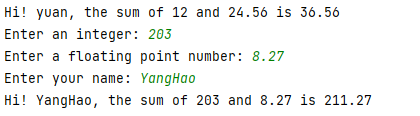
\includegraphics[width = 0.5\textwidth]{../pic/0.png}
    \caption{Problem0}
\end{figure}


\vspace{-3cm}\chapter{题目1:创建一个用来表示时间的类}

\section{1.1 题目}
\begin{enumerate}
    \item 创建一个用来存储时间数据的\lstinline{MyTime}类类型,当创建完这个类以后,应该保证下面的测试程序可以运行,且运行的结果如图所示。
    \begin{lstlisting}[
        language = Java,
        caption = {src/hw2/p1/TestTime.java, L5-L31}]
        // Official Test
        MyTime t1 = new MyTime();
        MyTime t2 = new MyTime(2);
        MyTime t3 = new MyTime(21, 34);
        MyTime t4 = new MyTime(12, 25, 42);
        MyTime t5 = new MyTime(t4);

        System.out.println("Constructed with:");
        System.out.println("t1: all arguments defaulted");
        System.out.printf(" %s\n", t1.toUniversalString());
        System.out.printf(" %s\n", t1.toString());
        System.out.println("t2: hour specified; minute and second defaulted");
        System.out.printf(" %s\n", t2.toUniversalString());
        System.out.printf(" %s\n", t2.toString());
        System.out.println("t3: hour and minute specified; second defaulted");
        System.out.printf(" %s\n", t3.toUniversalString());
        System.out.printf(" %s\n", t3.toString());
        System.out.println("t4: hour, minute and second specified");
        System.out.printf(" %s\n", t4.toUniversalString());
        System.out.printf(" %s\n", t4.toString());
        System.out.println("t5: MyTime object t4 specified");
        System.out.printf(" %s\n", t5.toUniversalString());
        System.out.printf(" %s\n", t5.toString());
        // when initialize t6 with invalid values,please output error information
        MyTime t6 = new MyTime(15, 74, 99);
        System.out.println("t6: invalid values");
        System.out.printf("%s\n", t6.toUniversalString());
    \end{lstlisting}
    \begin{figure}[H]
        \centering
        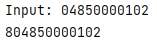
\includegraphics[width = 0.5\textwidth]{../pic/1/1.1.png}
        \caption{运行结果样例}
    \end{figure}
    \item 为\lstinline{MyTime}类增加三个成员方法:
    \begin{lstlisting}[language = Java]
    public void incrementHour();
    public void incrementMinute();
    public void incrementSecond();
    \end{lstlisting}
    每个方法都是在原有的对应数据上进行加1操作,但是一定要注意这种对时间的加1操作的合法性,比如考虑如下场景:\lstinline{MyTime}对象
    中的\lstinline{second}值为59,
    此时调用\lstinline{incrementSecond()}方法之后,\lstinline{second}值会成为0,同时\lstinline{minute}值也应该加1。
    将所有的特殊情况都考虑全面,并给出测试类。
\end{enumerate}


\section{1.2 题目分析}

本题需要对着已有的测试设计编写\lstinline{MyTime}类,并对\lstinline{increment}系列函数编写测试。

\begin{itemize}
    \item \textbf{Field}. 参照代码注释可知,可以定义三个\lstinline{int}变量\lstinline{hour}
        ,\lstinline{minute},\lstinline{second}分别代表小时、分钟、秒钟,24小时制。
    \item \textbf{Constructor Method}. 测试代码中一共出现了5种构造方法
    \begin{itemize}
        \item \lstinline{MyTime()},\lstinline{MyTime(int)},\lstinline{MyTime(int, int)},
        \lstinline{MyTime(int, int, int)};这4种构造方法都是直接将参数赋给类的变量,分别为
        默认、只赋时钟、只赋分钟、全赋值,未赋值的变量默认值为0;
        \item \lstinline{MyTime(MyTime)}这一构造方法是将参量复制给新的对象,即复制参量中的三个变量给新的对象。
        \item 值得注意的是,除了默认的构造方法外,构造方法均可以通过调用其他的构造方法实现,这样可以极大减少代码量,提高代码复用性。
    \end{itemize}
    \item \textbf{Other Method}. 本题目共要求实现编写5个实例化方法
    \begin{itemize}
        \item \lstinline{String toUniversalString()}. 本方法需要先判断\lstinline{this}数据是否合法,根据判断结果返回相应的字符串。
        \begin{enumerate}
            \item 判断\lstinline{this}的数据是否合法,因为错误信息需要检查所有的数据,所以设置一个初值为
                \lstinline{true}的\lstinline{boolean}变量\lstinline{flag},在判断过程中任一的判断错误
                都要将\lstinline{flag}置为\lstinline{false}.
            \item 如果不合法,输出判断过程中生成的错误信息
            \item 如果合法,根据\lstinline{this}的数据输出时间信息。此处需要注意字符串的输出格式:前导空格和Java format中的\lstinline{%02d}. 
        \end{enumerate}
        \item \lstinline{String toString()}. 本方法只需返回12小时制的时间字符串,所以只需注意\lstinline{hour}数据的处理和格式问题。
        \begin{enumerate}
            \item 参看测试代码可知,如果\lstinline{hour%12}为0,我们需要输出为12点,其他情况取余即可
            \item 格式问题可以参照上一个方法中的第三条,并在最后附上\lstinline{AM}/\lstinline{PM}
        \end{enumerate}
        \item \lstinline{increment}系列方法. 这几个方法逻辑基本类似,都是判断数据\lstinline{++}后是否超过上界,如果越界了需要将该数据置为0,
        并将更高级的单位数据\lstinline{++}。
        \begin{itemize}
            \item 基于这种\lstinline{++}操作的传递性,我们可以通过调用上一级单位的\lstinline{increment}方法简化我们的代码逻辑。
        \end{itemize}
    \end{itemize}
    \item \textbf{Test for Increment}. 测试代码只需确定每个\lstinline{increment}函数都正确无误,并测试其易错的进位即可,根据这个思路设计
        \lstinline{01:02:03}和\lstinline{23:59:59}. 
    两个数据。
    
\end{itemize}

\section{1.3 结果展示}

\begin{figure}[H]
    \centering
    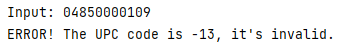
\includegraphics[width = 0.5\textwidth]{../pic/1/1.4.png}
    \caption{运行结果}
\end{figure}

\section{1.4 主干代码}

\begin{lstlisting}[
    language = Java,
    caption = {MyTime.java L8-L87}]
    public class MyTime {
    int hour;
    int minute;
    int second;

    MyTime() {
        hour = 0;
        minute = 0;
        second = 0;
    }

    MyTime(int h) {
        this();
        hour = h;
    }

    public MyTime(int h, int m) {
        this(h);
        minute = m;
    }

    public MyTime(int h, int m, int s) {
        this(h, m);
        second = s;
    }

    public MyTime(MyTime t4) {
        this(t4.hour, t4.minute, t4.second);
    }

    boolean ValidJudge(int num) {
        return num < 0 || num >= 60;
    }

    public String toUniversalString() {
        boolean flag = true;
        String s = "";

        if (ValidJudge(hour)) {
            flag = false;
            s += "hour must be 0-23\n";
        }
        if (ValidJudge(minute)) {
            flag = false;
            s += "minute must be 0-59\n";
        }
        if (ValidJudge(second)) {
            flag = false;
            s += "second must be 0-59\n";
        }
        if (flag) return String.format("   %02d:%02d:%02d", hour, minute, second);
        else return s;
    }

    @Override
    public String toString() {
        String s;
        s = (hour % 12 == 0) ? String.format("   %02d:%02d:%02d ", 12, minute, second) :
                String.format("   %02d:%02d:%02d ", hour % 12, minute, second);
        s += (hour < 12) ? "AM" : "PM";
        return s;
    }

    public void incrementHour() {
        if (++hour >= 24) hour = 0;
    }

    public void incrementMinute() {
        if (++minute >= 60) {
            minute = 0;
            incrementHour();
        }
    }

    public void incrementSecond() {
        if (++second >= 60) {
            second = 0;
            incrementMinute();
        }
    }
\end{lstlisting}

\begin{lstlisting}[
    language = Java,
    caption = {TestTime.java L33-L46}]
    // My Test for new increment methods
        System.out.println("-----NEW TESTS FOR INCREMENT-----");
        MyTime t7 = new MyTime(1,2,3);
        System.out.printf("t7 is initialized as %s\n",t7.toUniversalString());
        t7.incrementHour();
        System.out.printf("  after t7.incrementHour(), t7 is %s\n", t7.toUniversalString());
        t7.incrementMinute();
        System.out.printf("  after t7.incrementMinute(), t7 is %s\n", t7.toUniversalString());
        t7.incrementSecond();
        System.out.printf("  after t7.incrementSecond(), t7 is %s\n", t7.toUniversalString());
        MyTime t8 = new MyTime(23, 59, 59);
        System.out.printf("t8 is initialized as %s\n",t8.toUniversalString());
        t8.incrementSecond();
        System.out.printf("  after t8.incrementSecond(), t8 is %s\n", t8.toUniversalString());
\end{lstlisting}

\section{1.5 总结与收获}

本题目较为简单,但其中蕴含的方法间互相调用以提高代码复用率的思想让我收益良多。

本题中的输出涉及大量关于细节,包括:如何让代码的逻辑更舒服更“美”、java字符串的format形式等等,这些细节虽然加起来不到三五行,却占据了我
50\%以上的时间,尤其是对代码逻辑的优化和打磨需要反复斟酌。

% 1、题目
% 2、数据设计
% 3、算法设计
% 4、主干代码说明
% 5、运行结果展示
% 6、总结和收获
\vspace{-3cm}\chapter{实验2:Linux文件管理}

\section{2.1 实验目的}

% 熟练掌握Linux操作系统的使用,掌握Linux的系统的进程管理和文件管理功能。
% 实验要求:
% 完成实验内容并写出实验报告,报告应具有以下内容:
% 1)	实验目的;
% 2)	实验内容;
% 3)	题目分析及基本设计过程分析;
% 4)	配置文件关键修改处的说明及运行情况,应有必要的效果截图;
% 5)	实验过程中出现的问题及解决方法;
% 6)	实验体会。

\section{2.2 实验内容}

\begin{enumerate}
    \item 将若干已有用户加入到同一个组xjtuse中。在/home下创建一个共享的公用目录public,
        允许xjtuse组中的用户对该目录具有读写和执行操作。(给出相关命令及运行结果)
    \item 对于public目录下的文件,只有文件的拥有者才具有删除文件的权限。(给出相关命令及运行结果)
    \item 对于public目录下的文件,也可以通过路径/mnt/public来访问。(给出相关命令及运行结果)
    \item 看Linux系统磁盘空间的使用情况(给出显示结果),并为/分区创建磁盘配额,
        使得用户可用空间的软限制为100M,硬限制为150M,且每个用户可用的inodes的软限制为100,
        硬限制为120。并对磁盘配额情况进行验证测试。(给出相关命令及运行结果)
\end{enumerate}

\section{2.3 题目分析}

\begin{enumerate}
    \item 通过实验一的知识即可实现用户加入同一组,通过chown、chgrp、chmod等指令即
        可更改public的所属人,所属组和权限。
    \item 
\end{enumerate}




\vspace{-3cm}\chapter{实验3. 长度n的子序列最大乘积}

\section{3.1 题目}
\textbf{从文件中输入}一个数字序列字符串,计算给定的长度\lstinline{n}的子序列中的最大乘积值。

例如:如果输入“1027839564”,指定长度为3的最大子序列乘积值为 $270 = 9\times 5\times 6$;
指定长度为5的最大子序列乘积值为$7560=7\times 8\times 3\times 9\times 5$。

备注:
\begin{enumerate}
    \item 数字序列字符串的最大长度\lstinline{maxLength}的范围为:[1……1000];
    \item \lstinline{n}的取值范围为[1……\lstinline{maxLength}-1];
    \item 程序要注意处理边界情况;
    \item 程序的输入数据必须从文件中读取。
\end{enumerate}

下图为一个长度为1000的字符串数字序列,在这个序列中,长度为4的最大子序列乘积为 $5832 = 9\times 9\times 8\times 9$. 
\begin{figure}[H]
    \centering
    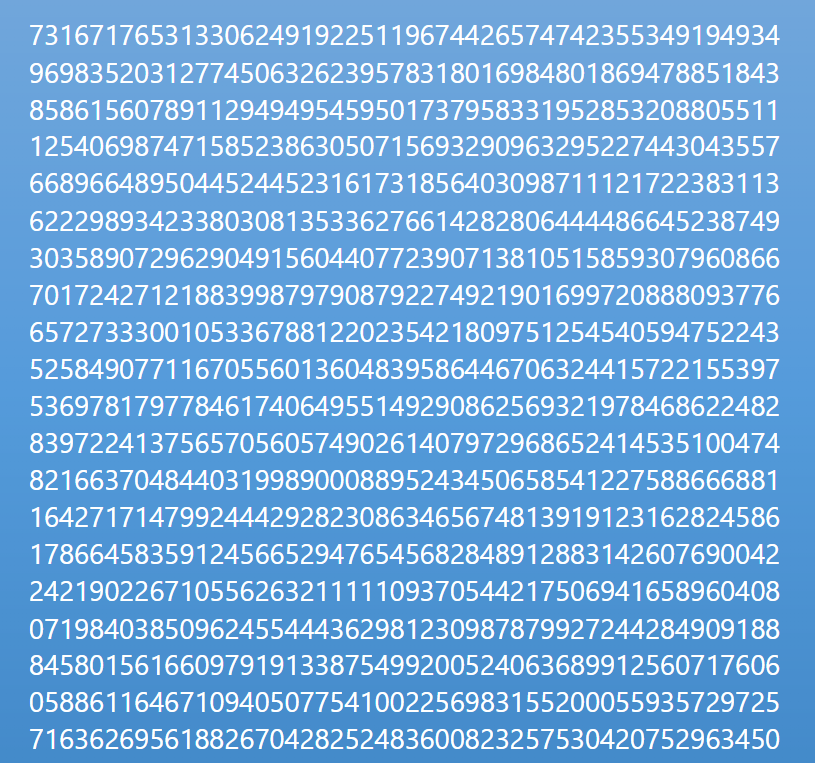
\includegraphics[width = 0.8\textwidth]{../pic/3/3.0.png}
\end{figure}

\section{3.2 思路分析}

题目本身很简单,解决和验证思路可以分为三部分
\begin{enumerate}
    \item \textbf{数据输入}. 
        \begin{itemize}
            \item 题中要求从文件输入,我们将数据存放在input文件夹的input3.txt中;
            \item 考虑到数据的长度,只能以字符串的形式输入,并通过Problem1中提到过的库函数以数组的方式处理数据。
        \end{itemize}
    \item \textbf{算法设计}. 只需要从第[0……n-1]位开始向后逐位扫描即可,但考虑到n位数相乘可能大于int甚至long类型的边界,综合
        考虑并查阅资料后,决定采用\lstinline{Math}库里的\lstinline{BigInteger}这个类. 下面对未采用的优化方案做出解释。
        \begin{itemize}
            \item 高精度. 即用\lstinline{String}模拟高位数乘法的过程。而实际上\lstinline{BigInteger}类已经帮我们内部实现了这一点,
                而且配有丰富的函数和数值优化,这一定是比我们自己写更快更方便的。
            \item 记忆组中的最小值,如果下一个比这个小就可以直接跳过。这一步看似优化了一步,实际上增加了比较的环节,从算法复杂性分析来看
                并没有优化。
        \end{itemize}
    \item \textbf{数据测试}. 本题思路简单,用题中所给数据验证即可
\end{enumerate}

\section{3.3 代码展示}

为了便于验证,用一个循环来模拟不断查询新的最大子序列

\lstinputlisting[
    language = Java,
    caption = {\bf Problem3.java}
    ]{../../../ProblemSet/src/Problem3.java}

\section{3.4 结果展示}

输入数据采用题目中的“1000位数据”,并设置三种长度

\begin{figure}[H]
    \centering
    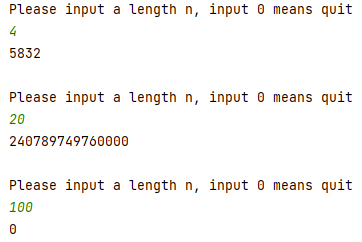
\includegraphics[width = 0.4\textwidth]{../pic/3/3.1.png}
\end{figure}

\section{3.5 总结与收获}

第一次看到本题时我想到了3.2中所写的一些思路,苦恼于怎么优化其时间复杂度以及优雅地写出来。
并不知道也没有打算使用BigInteger但后来认真分析,查阅JDK的官方文档和BigInteger的实现原理后
意识到BigInteger这个类的便捷性和性能远比自己写的好,

“如果你不知道为什么要优化,那这样的优化毫无意义(not make sense at all)” 

\rightline{—— Professor.Weaver (UC.Berkeley)}
\vspace{-3cm}\chapter{The Basic Idea of Java OOP}

考虑到作业需要的是一份内容总结,而非讲义,故内容编排上和教学顺序有一定出入。

\section{0x00 基本概念}

重载(overload):作为一门现代化的语言,Java支持方法重载,即:只要方法名和参数类型不全相同即可视作一个新的方法。重载方法的原则遵循就近原则。

强制类型转换(cast):Java也支持变量强制类型转换,注意:这种转换只是一种对编译器的“欺骗”——即告诉编译器这一块为类型转换的目标类型。

Java中一切非原始类型的都以引用类型在程序中存在。

Java中每个引用变量有两个类型:
\begin{itemize}
    \item 静态类型:声明时定义的类型,在编译时确定并检查,也就是说cast改变的是那一块的静态类型。
    \item 动态类型:变量实际指向的类型,在运行时确定。
\end{itemize}

Java中用final关键字表示常量

\section{0x01 类}

Java中的一切函数(方法)、变量和代码都是在一个个类中。

自然而然地,由基本的面向对象思想,一个类可以被另一个类所继承,Java中用extends关键词。
\begin{lstlisting}[language = Java]
    public subClassA extends parentClassB{
        // ... 
    }
\end{lstlisting}

子类会继承父类的所有变量和方法,可以通过 super 调用形成独一无二的“is a”关系

每个类都有变量(Field)和函数(Method)两部分,类中成员的声明需要访问权限修饰符,修饰符主要在其他类调用该类中的成员时确认合法性,
Java中共有四种修饰符,各自含义如下:
\begin{table}[H]
    \centering
    \begin{tabular}{|c|c|c|c|c|}
        \hline
        \textbf{访问范围} & \textbf{private} & \textbf{friendly(默认)} & \textbf{protected} & \textbf{public} \\ \hline
        同一个类          & √                & √                     & √                  & √               \\ \hline
        同一个包中的其他类     & ×                & √                     & √                  & √               \\ \hline
        不同包中的子类       & ×                & ×                     & √                  & √               \\ \hline
        不同包中的非子类      & ×                & ×                     & ×                  & √               \\ \hline
    \end{tabular}
\end{table}


\subsection{abstract\& final}
abstract: 
\begin{itemize}
    \item abstract修饰的方法可以不定义,只能存在于abstract类中
    \item abstract修饰的类不能被直接实例化,类中可以存在非abstract方法
\end{itemize}

final: final修饰的类不能被继承,final修饰的方法也不能进行修改。


\section{0x02 接口}

由于Java只支持类对类的单继承,为了使继承更加地灵活,除了类,Java中还存在另一种和类相似的类型:接口。
接口需要定义方法,但不实现方法(不过随着Java版本的更新也有了default的方法实现)。

当一个类需要继承这个接口时,声明类时采用implements关键词,用法与extends类似。但一个类可以继承多个接口,接口与接口用逗号隔开。
\begin{lstlisting}[language = Java]
public subClassA extends parentClassB implements InterfaceA, InterfaceB{
    // ... 
}
\end{lstlisting}

如果一个类继承了某个接口,则它一定要实现接口中的所有方法。

类和接口不存在is a的关系。

考虑到接口可以独立作为一个类型,也可以被实现,后文的叙述中涉及继承的部分默认也适用于继承自接口。

\section{0x03 继承}

继承的思想很好理解和接受,但继承中存在大量细节需要说明和理解记忆。

\subsection{3.0 Constructor}

子类的构造方法的第一句必须是父类的构造方法,这一句也可以通过调用子类的其他构造方法以实现。

如果构造方法的第一句和上述不符,编译器会在第一句插一条父类的默认构造方法 super() ,如果父类没有默认的构造方法此处会编译报错。

\subsection{3.1 Override}

当子类中的某个\textbf{方法}和父类的方法名相同,修饰符访问范围更开放,且参数类型也相同时,我们称该方法覆盖(override)了父类中的原方法,
此时若想通过子类调用父类方法只能通过super()。

\subsubsection{override 流程}
\begin{enumerate}
    \item 当且仅当\textbf{方法}参数类型和方法名均相同时会被认为是override,开始检查override的合法性
    \item 当方法名和参数类型均相同,但返回值不同或访问权限更小,这个函数不合法,会出现编译错误
\end{enumerate}

\begin{figure}[H]
    \centering
    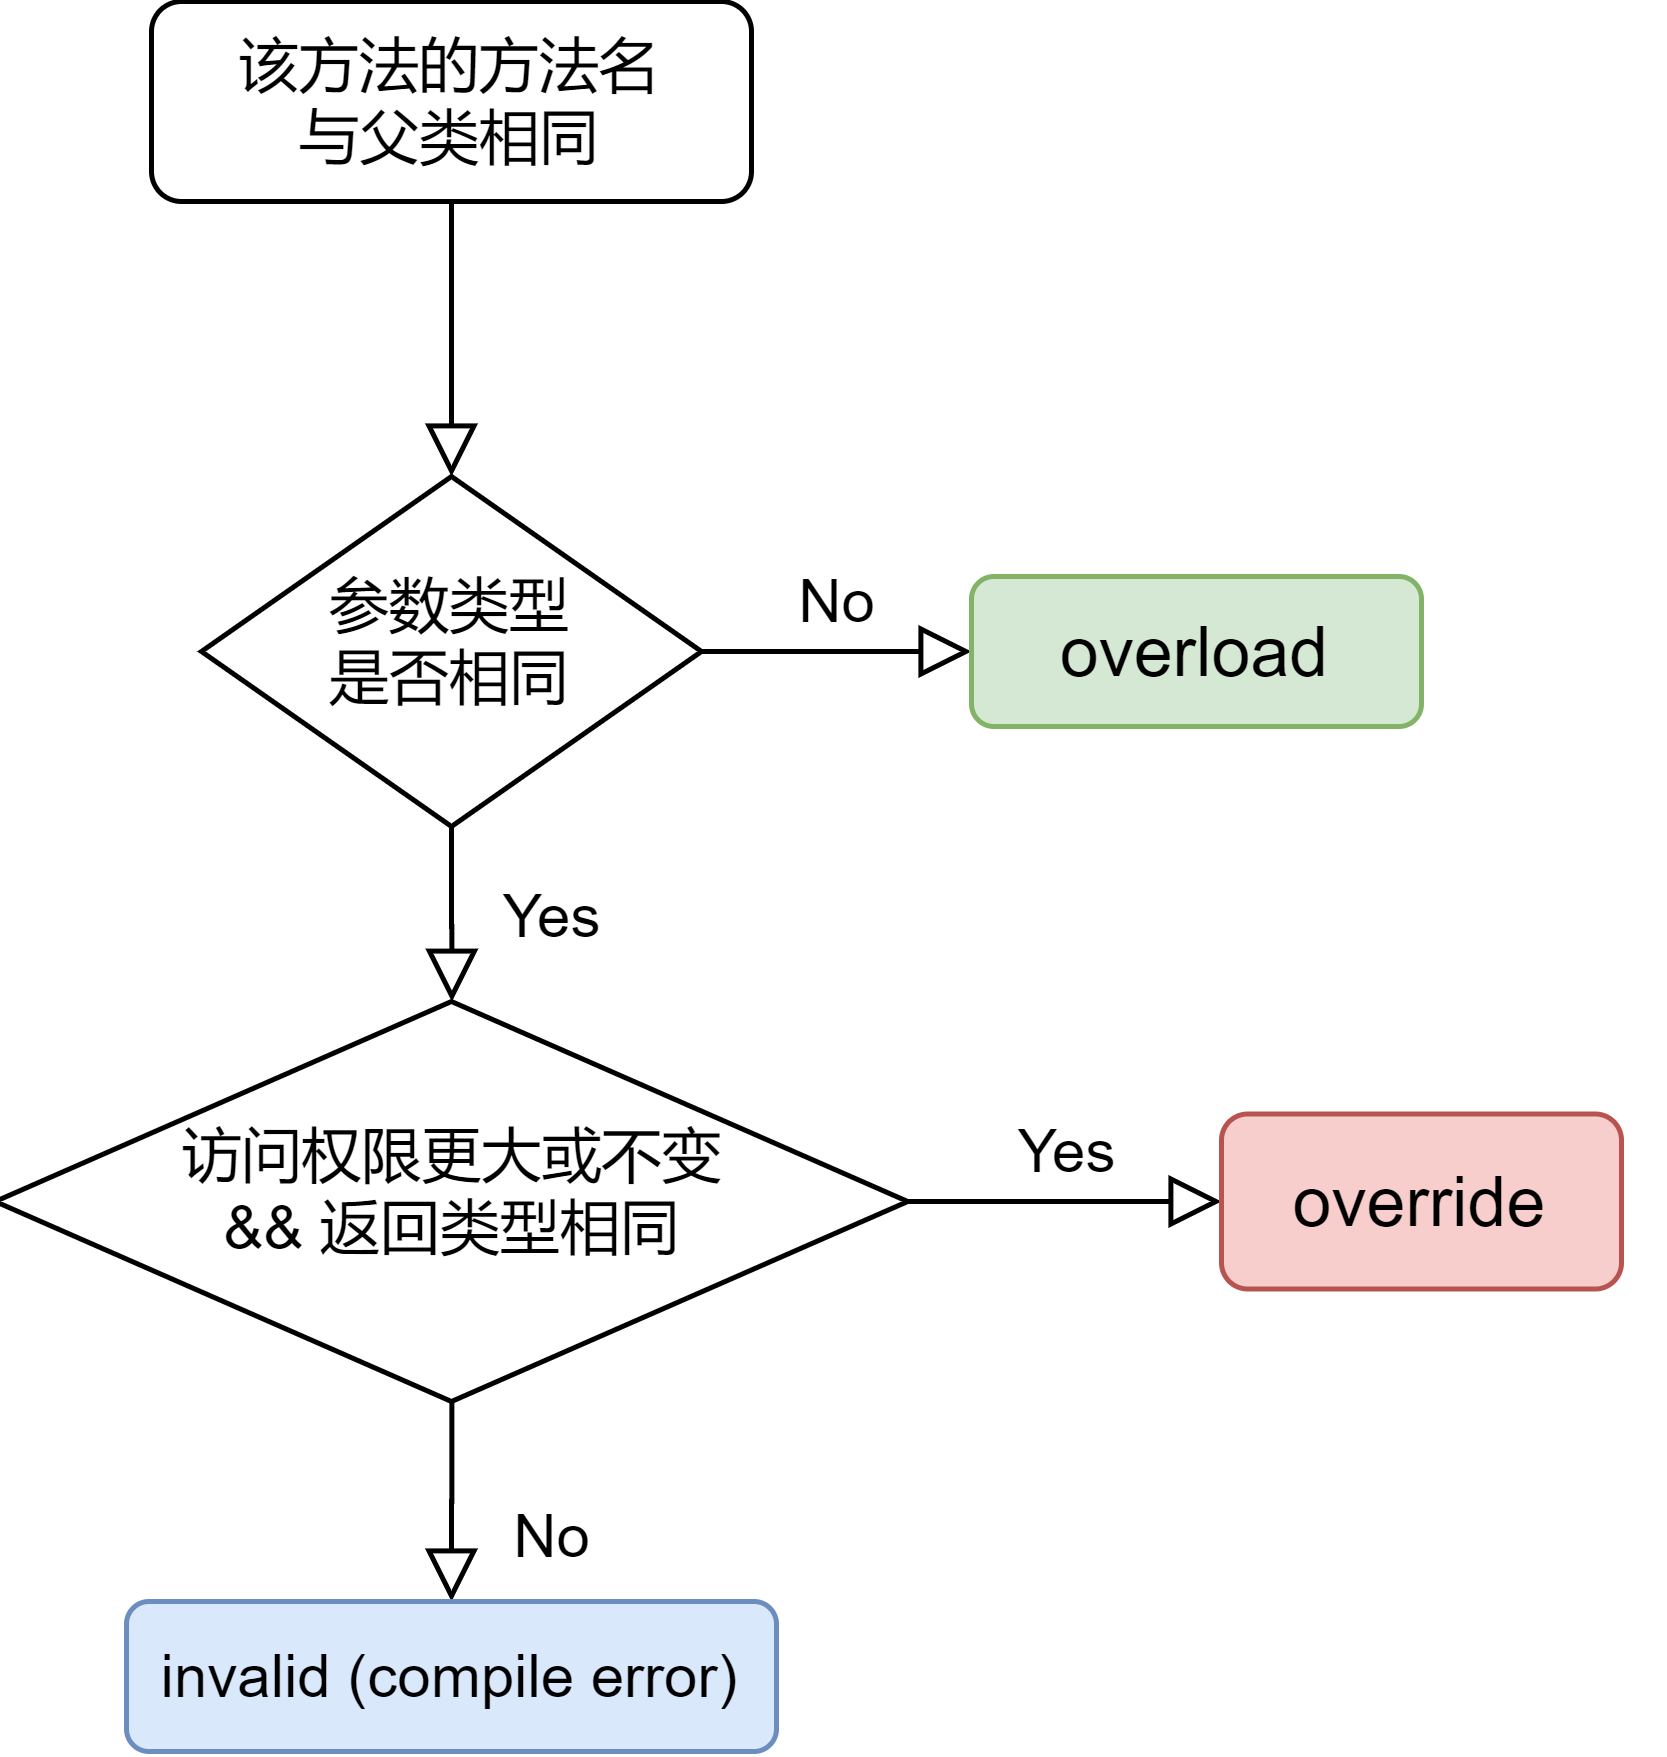
\includegraphics[width = 0.6\textwidth]{../pic/4/flowchart_override.png}
\end{figure}

\subsubsection{add \& override}

\textbf{\color{red}{变量中不存在覆盖的概念,如果变量出现重名,会新增一个变量。}}

如果出现重载,会新增一个方法。

\subsection{3.2 Check\& Selection}

从编译的角度看:在编译过程中需要检查程序中每一句的合法性,这时只能采用静态类型确认,对静态类型来说不合法就会报错。

\subsubsection{cast \& type}

有了继承的概念,我们可以先对cast的概念在继承的角度作进一步的说明。

编译时:当两个对象的类之间存在继承关系时可以cast,否则会出现compile error

运行时:如果对象的动态类型并非cast的结果,则会出现exception. 从继承关系上看,向上转换可以毫无顾忌地执行
(因为有“is a”关系),但向下转换时需要谨慎考虑。

\subsubsection{Variable field}

在java的类中,变量域依赖于静态类型而存在。

因此,如果需要不利用super访问父类的变量也可以利用cast转为父类再访问变量。

\subsubsection{Method}

除了实例方法外,类中的数据成员和类方法均依赖于对象的静态类型存在,也就是说在编译时就确定了要用哪个数据/方法。

实例方法比较特殊,采用一种动态选择的机制,在运行时才会依据引用变量指向的实例对象类型选择要执行的方法。

\section{0x04 Examples}

上述的概念尤其是3.2部分存在一定的抽象性,没有陷进坑里过很难一次性想明白,故提供几个样例程序如下

\lstinputlisting[language = Java, caption = {Bird.java}]{../../../ProblemSet/src/hw2/p4/Bird.java}

\lstinputlisting[language = Java, caption = {Dog.java}]{../../../ProblemSet/src/hw2/p4/Dog.java}

根据以上两个代码可以对下面这段代码有更好的理解
\lstinputlisting[language = Java, caption = {Supplier.java}]{../../../ProblemSet/src/hw2/p4/Supplier.java}

\section{0x05 Polymorphism}

什么是多态?

从程序到进程周期的角度看,Java中存在两种多态:

\begin{itemize}
    \item 静态多态(编译时多态性):同名方法可以有多个,在编译时能够确定执行同名方法中的哪一个,则称为编译时多态性.
    \item 动态多态(运行时多态):由于覆盖的影响,在编译时不能确定,只能在运行时才能确定执行多个同名方法中的哪一个,则称为运行时多态性.
\end{itemize}

从类的角度看,Java 中也存在类多态:

\begin{itemize}
    \item 方法重载:同一个类的同名方法可以重载;
    \item 子类重定义:子类可以重定义父类的成员,从而隐藏变量或者覆盖方法
\end{itemize}
\vspace{-3cm}\chapter{实验5. 直方统计图}

\section{5.1 题目}
 
编写一个程序,从文件中读入不定个数的数据。每个数据都已空格或者回车分割,每个数的大小都在[0..100]之间,统计10
个区间的数据的个数,并以两种方式将统计结果进行展示:水平直方图和垂直直方图。示例图如下:(测试数据自行准备)

\begin{figure}[H]
    \centering
    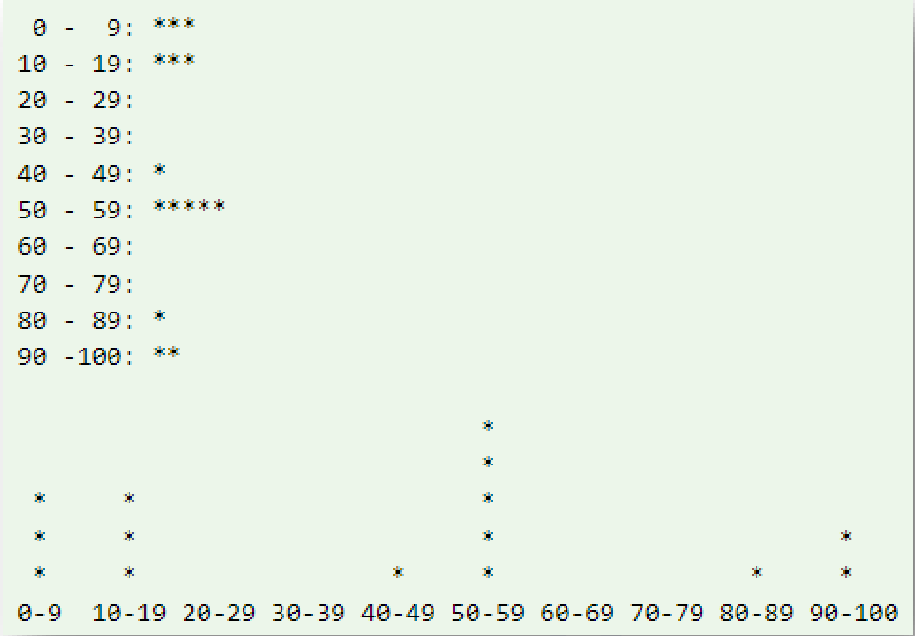
\includegraphics[width = 0.7\textwidth]{../pic/5/5.0.png}
\end{figure}

\section{5.2 思路分析}

本题可分为四个模块。
\begin{enumerate}
    \item \textbf{数据输入}. 为了优雅方便地测试和生成数据,我们采用\lstinline{Random}类批量生成并存储在\lstinline{input/input5.txt}中
        \begin{itemize}
            \item 最常用的是Random中的\lstinline{public int nextInt(int origin, int bound)}这一函数,该函数会返回一个
                [\lstinline{origin}, \lstinline{bound})之间的整数,下文分别简称为上界和下界;
            \item 题目未要求数据的个数。考虑到题目的相关要求,决定把以下界为50,上界为101随机得到一个数据个数;
            \item 每个数据以下界为0,上界为101随机生成,用回车分割并通过\lstinline{BufferedWriter}类(需要
                \lstinline{throw IOException})写入到文件中。
        \end{itemize}
    \item \textbf{数据读取与统计}. 用一个长度为10的整型数组(\lstinline{stat})存储十个部分各自出现的频次。
        \begin{itemize}
            \item 因为数据个数不确定,所以需要\lstinline{hasNext()}确定。
            \item 从文件中读取数据时可以读取每个数据后直接将数据\lstinline{/10},然后将对应的数组中的数\lstinline{+1}。
                需要为100设置一个特例。
        \end{itemize}
    \item \textbf{水平直方图打印}. 对每一行只需在第i行:
        \begin{enumerate}
            \item 打印各自的前缀,第一行和最后一行设置一个特例;
            \item 打印\lstinline{stat[i]}个\lstinline{*}并打印回车;
        \end{enumerate}
    \item \textbf{垂直直方图打印}. 参考Problem4中以像素矩阵的角度打印。
        \begin{enumerate}
            \item 首先遍历数组得到最大值以确定这个矩阵的高度;
            \item 不用把每个打印都看作一个像素,而是把每一部分看作像素,经过这样分割后只需观察每个像素内打印空格的规律;
            \item 对每一行刚开始的时候打印一个空格作为特例,为了保证输出的正确性最后一次打印后即回车;
            \item 最后一行需要输入每个部分的表示。
        \end{enumerate}
\end{enumerate}

\section{5.3 代码与测试}

本题代码完全参照5.2中的思路,实现较为简单,具体可翻阅附录。

本题重在打印出的形式是否正确对应,所以随机打印即可。

\section{5.4 运行结果}

运行结果如下

\begin{figure}[H]
    \centering
    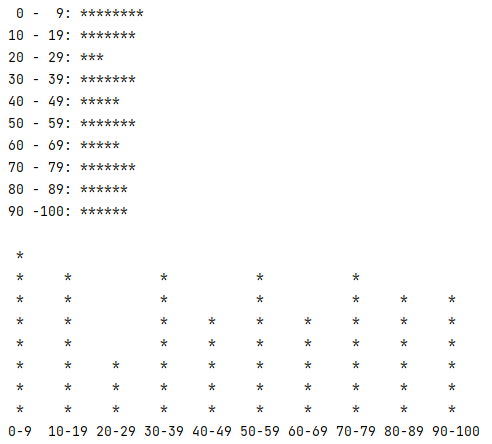
\includegraphics[width = 0.5\textwidth]{../pic/5/5.1.png}
\end{figure}

\section{5.5 总结与收获}

本题比较简单,只是有点繁琐,但需要考虑到设置范围的问题。其次需要从题目给定的样例中总结打印的规律,并把这个规律转换成打印时的一个个单元处理。

第一遍写代码时没有采用\lstinline{hasNext()},运行出现了问题,这说明我对文件输入依旧比较陌生;也没有采用即读即记录,而是打算先存储到
\lstinline{Vector}中,
以后写代码一定要下意识思考优化问题,但也不能看到什么都想到优化。
\vspace{-3cm}\chapter{实验6. 蒙特·卡洛方法模拟}

\section{6.1 题目}

编写一个程序来模拟蒙特卡罗方法。具体的过程可以按照下面的方式来模拟:如下图所示(a)中的正方形,假设向正方形
所代表的区域投掷飞镖,如果投掷100000次,那么飞镖落在奇数数字所对应区域的概率是多少呢? 

\begin{figure}[H]
    \centering
    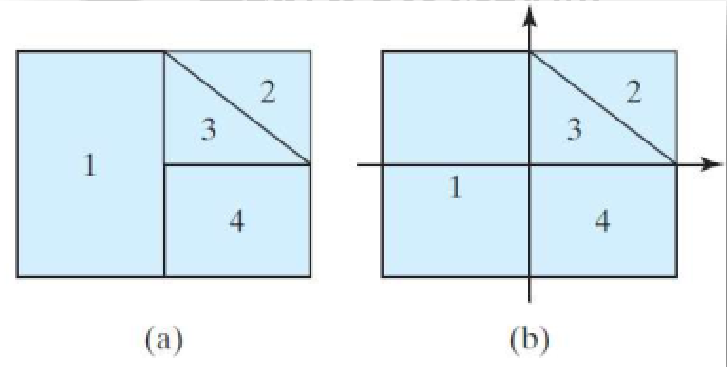
\includegraphics[width = 0.8\textwidth]{../pic/6/6.0.png}
\end{figure}

提示:可以将(a)图放到如(b)所展示的坐标系中,程序随机的在整个区域中生成点,这样模拟投掷飞镖的行为。

\section{6.2 思路分析}
\begin{enumerate}
    \item 如题目中提示所说,可以如b图所示建立坐标系,程序随机地在区域中生成点(即生成两个范围内的数作为横纵坐标)
    \item 为了模拟更精确,随机生成
        应该采用\lstinline[language = Java]{double nextDouble(double origin, double bound)}随机生成小数。
        代码中设正方形的范围为$[-100,100]\times[-100,100]$。
    \item 每次生成后需要判断该点是否在奇数数字,即1、3区域,通过简单的平面几何相关知识即可确定。如果在就将用来记录次数的变量+1。
    \item 随机生成100000次结束后输出记录次数的变量/100000的值,此处需要注意的是需要强制转换为double否则会自动转为整型。
\end{enumerate}

\section{6.3 代码与结果展示}

代码如下

\lstinputlisting[
    language = Java,
    caption = {\bf Problem6.java}
]{../../../ProblemSet/src/Problem6.java}

结果如下

\begin{figure}[H]
    \centering
    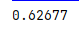
\includegraphics[width = 0.15\textwidth]{../pic/6/6.1.png}    
\end{figure}

\section{6.3 总结与收获}

本题看似简单但输出有一个大坑,即强制转换,很久没使用我几乎已经遗忘了这个性质

本题的名字看似唬人,但题目难度很低,不要被吓到,仔细阅读要求即可
%%% Appendix
\chapter{附录 代码与运行结果汇总}

\section{实验0. 通过键盘输入和文件输入}

\lstinputlisting[
        language = Java,
        caption = {\bf Problem0.java}    
]{../../../ProblemSet/src/Problem0.java}

\begin{figure}[H]
    \centering
    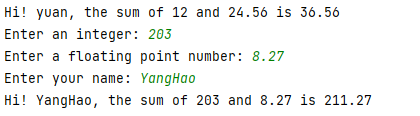
\includegraphics[width = 0.5\textwidth]{../pic/0.png}
    \caption{实验0运行结果}
\end{figure}

\newpage
\section{实验1. UPC码}

\lstinputlisting[
        language = Java,
        caption = {\bf Problem1.java}    
]{../../../ProblemSet/src/Problem1.java}

\begin{figure}[H]
	\centering
	\begin{subfigure}{0.325\linewidth}
		\centering
		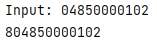
\includegraphics[width=0.7\linewidth]{../pic/1/1.1.png}
	\end{subfigure}
	\begin{subfigure}{0.325\linewidth}
		\centering
		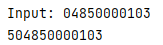
\includegraphics[width=0.7\linewidth]{../pic/1/1.2.png}
	\end{subfigure}
	\begin{subfigure}{0.325\linewidth}
		\centering
		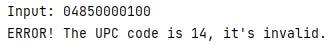
\includegraphics[width=1\linewidth]{../pic/1/1.3.png}
	\end{subfigure}
    \vspace{1cm}
    \begin{subfigure}{0.325\linewidth}
		\centering
		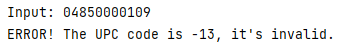
\includegraphics[width=1\linewidth]{../pic/1/1.4.png}
	\end{subfigure}
	\begin{subfigure}{0.325\linewidth}
		\centering
		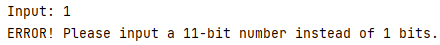
\includegraphics[width=1\linewidth]{../pic/1/1.5.png}
	\end{subfigure}
	\begin{subfigure}{0.325\linewidth}
		\centering
		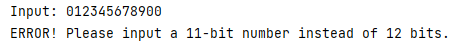
\includegraphics[width=1\linewidth]{../pic/1/1.6.png}
	\end{subfigure}
    \vspace{1cm}
    \begin{subfigure}{0.325\linewidth}
		\centering
		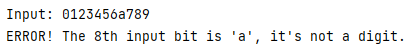
\includegraphics[width=1\linewidth]{../pic/1/1.7.png}
	\end{subfigure}
	\begin{subfigure}{0.325\linewidth}
		\centering
		
\includegraphics[width=1\linewidth]{../pic/1/1.8.png}
	\end{subfigure}
	\begin{subfigure}{0.325\linewidth}
		\centering
		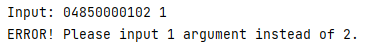
\includegraphics[width=1\linewidth]{../pic/1/1.9.png}
	\end{subfigure}
	\caption{Output of Problem1}
\end{figure}

\newpage
\section{实验2. 数字转英语}

    \lstinputlisting[
        language = Java, 
        caption = {\bf Problem2.java}
    ]{../../../ProblemSet/src/Problem2.java}

    \begin{figure}[H]
        \centering
        \begin{subfigure}{0.13\linewidth}
            \centering
            
\includegraphics[width=0.5\linewidth]{../pic/2/2.1.png}
            \caption{input: 0}
        \end{subfigure}
        \begin{subfigure}{0.17\linewidth}
            \centering
            
\includegraphics[width=1\linewidth]{../pic/2/2.2.png}
            \caption{input: -1}
        \end{subfigure}
        \begin{subfigure}{0.17\linewidth}
            \centering
            
\includegraphics[width=1\linewidth]{../pic/2/2.3.png}
            \caption{input: 100}
        \end{subfigure}
        \begin{subfigure}{0.17\linewidth}
            \centering
            
\includegraphics[width = 1\linewidth]{../pic/2/2.4.png}
            \caption{input: 1000}
        \end{subfigure}
        \begin{subfigure}{0.27\linewidth}
            \centering
            
\includegraphics[width=1\linewidth]{../pic/2/2.5.png}
            \caption{input: 5000210}
        \end{subfigure}
        \begin{subfigure}{1\linewidth}
            \centering
            
\includegraphics[width=0.9\linewidth]{../pic/2/2.6.png}
            \caption{input: 999999999}
        \end{subfigure}
        \caption{Output of Problem2}
    \end{figure}

\newpage
\section{实验3. 长度n的子序列最大乘积}
    \lstinputlisting[
            language = Java, 
            caption = {\bf Problem3.java}
    ]{../../../ProblemSet/src/Problem3.java}
    \begin{figure}[H]
        \centering
        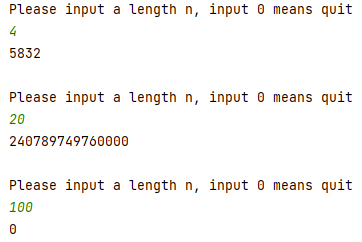
\includegraphics[width = 0.4\textwidth]{../pic/3/3.1.png}
        \caption{Output of Problem3}
    \end{figure}

\newpage
\section{实验4. 模式化打印图形}
    \lstinputlisting[
            language = Java, 
            caption = {\bf Problem4.java}
    ]{../../../ProblemSet/src/Problem4.java}
    \begin{figure}[H]
        \centering
        \begin{subfigure}{0.19\linewidth}
            \centering
            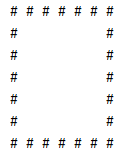
\includegraphics[width=1\linewidth]{../pic/4/4.a.png}
            \caption{input: a 7}
        \end{subfigure}
        \begin{subfigure}{0.19\linewidth}
            \centering
            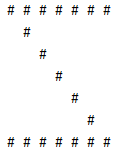
\includegraphics[width=1\linewidth]{../pic/4/4.b.png}
            \caption{input: b 7}
        \end{subfigure}
        \begin{subfigure}{0.19\linewidth}
            \centering
            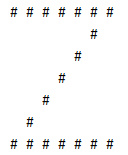
\includegraphics[width=1\linewidth]{../pic/4/4.c.png}
            \caption{input: c 7}
        \end{subfigure}
        \begin{subfigure}{0.19\linewidth}
            \centering
            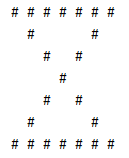
\includegraphics[width = 1\linewidth]{../pic/4/4.d.png}
            \caption{input: d 7}
        \end{subfigure}
        \begin{subfigure}{0.19\linewidth}
            \centering
            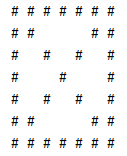
\includegraphics[width=1\linewidth]{../pic/4/4.e.png}
            \caption{input: e 7}
        \end{subfigure}
        \caption{Output of Problem4}
    \end{figure}

\newpage
\section{实验5. 直方统计图}
\lstinputlisting[
    language = Java, 
    caption = {\bf Problem5.java}
]{../../../ProblemSet/src/Problem5.java}
\begin{figure}[H]
    \centering
    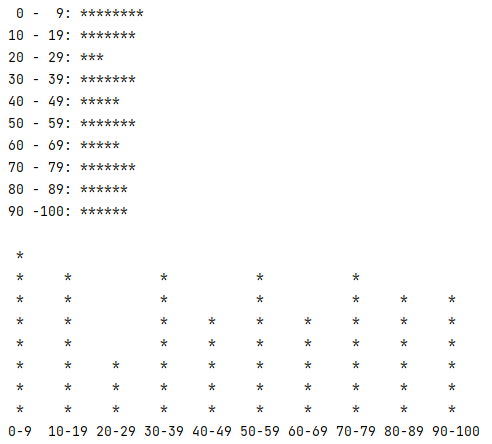
\includegraphics[width = 0.5\textwidth]{../pic/5/5.1.png}
    \caption{Output of Problem5}
\end{figure}

\newpage
\section{实验6. 直方统计图}
\lstinputlisting[
    language = Java, 
    caption = {\bf Problem6.java}
]{../../../ProblemSet/src/Problem6.java}
\begin{figure}[H]
    \centering
    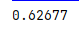
\includegraphics[width = 0.15\textwidth]{../pic/6/6.1.png}   
    \caption{Output of Problem6} 
\end{figure}
    

\chapter{参考文献}

\section{A. 解题内容参考}
\begin{itemize}
    \item[a.] Java® Platform, Standard Edition \& Java Development Kit Version 17 API Specification [DB/OL] \newline 
        \url{https://docs.oracle.com/en/java/javase/17/docs/api/index.html}, 2022. 
\end{itemize}

\section{B. \LaTeX~代码参考}
\begin{itemize}
    \item[b.] \href{https://zhuanlan.zhihu.com/p/385727082}{【LaTeX】自用简洁模板(六):学校作业} 
    \item[c.] \href{https://zhuanlan.zhihu.com/p/65441079}{LaTeX 里「添加程序代码」的完美解决方案}
\end{itemize}


\end{document}